Based on the problem formulation and the background research the following four hypothesis have been established:
\begin{enumerate}
\item Random Forest algorithm has a higher frequency of correctly classifying whales than Random Selection from images
\item Deep Neural Network algorithm has a higher frequency of correctly classifying whales than Random Selection from images
\item Having the knowledge of whales position in a given image increase the frequency of correctly classification of whales with Deep Neural Network
\item Having the knowledge of whales position in a given image increase the frequency of correctly classification of whales with Random Forest
\end{enumerate}

\subsection{Testing hypothesis}
The two first hypothesis can be tested in the same testing environment. This testing environment is described in Figure \ref{fig:environmentRaw}. The only difference between the tests of the two hypothesis is that the algorithm for building a model is changed.
For the test a threefold cross-validation is used, where the data set is split into three parts in equal size. Two of these parts are then used for training the prediction model. The last part is used to test the model, since the data used for training would be biased and therefore cannot be used. After the training and testing of a model the procedure is repeated two more time with different data parts as training and test. 
The result of these three rounds of test is then aggregated and compared to the result from a random selection, with the use of T-test to either rejecter or fail to reject the hypothesis.

\begin{figure}
\centering
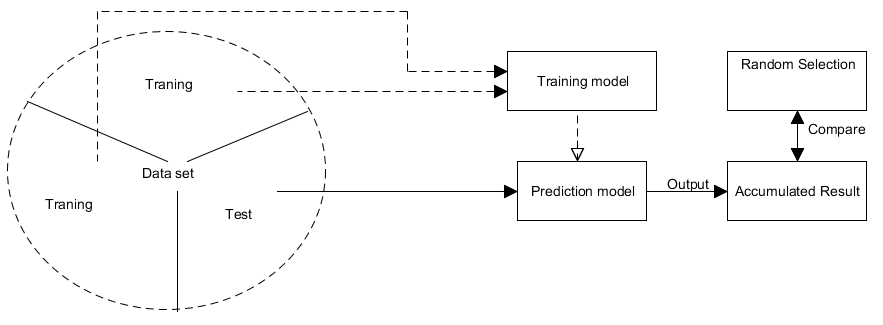
\includegraphics[width=\linewidth]{Images/EnvironmentOnRawData}
\caption{The environment when testing the first two hypothesis}
\label{fig:environmentRaw}
\end{figure}

For the second two hypothesis, the same procedure is used as for the first two, only with minor changes as seen from Figure \ref{fig:environmentPre}. The difference here is that both training and test set is pre processed to find the location of the whale and cropping the image to fit the whale.

\begin{figure}
\centering
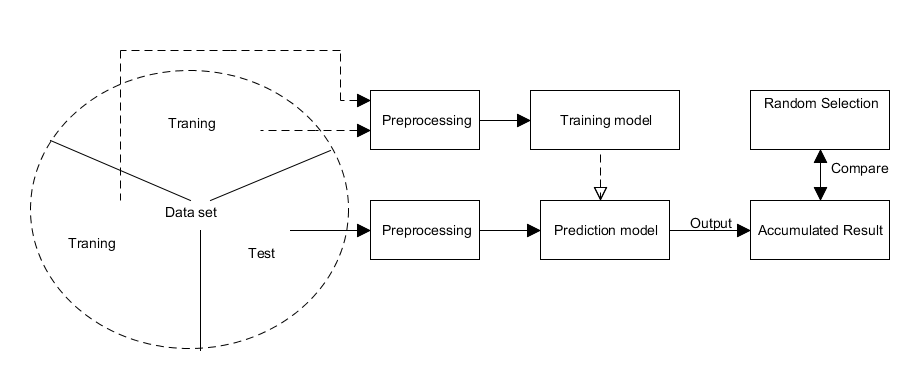
\includegraphics[width=\linewidth]{Images/EnvironmentWithPre}
\caption{The environment when testing the first two last hypothesis}
\label{fig:environmentPre}
\end{figure}